\providecommand{\main}{..}
\documentclass[\main/master.tex]{subfiles}
\begin{document}
\chapter{introduction}\label{chp:example-1}
\section{garvity measurement problem}

Gravitational field has a very unique nature compare to other fields. Gravitational field could not be shielded and the force could not be compensated. The Gravitational force is inverse to the square of the distance between the masses, causing a very weak force. Those properties makes it a dominating force in nature but very hard to measure at experiments.
\par
Since the invention of the first modern gravimeter, at 1936, gravimetry is used widely to exam matter properties or measure gravitational fields. Precision gravimetry \cite{Wahr04,Bingham10,Bell98,Leeuwen00,Diorio03,Romaides01,Peters01,Luther82,Kuroda95,Karagioz96,Bagley97,Gundlach00,Quinn01,Armstrong03,Kleinevoss99,Parks10,Peters99,Mcguirk02,Dimopoulos07,Lamporesi08,Sorrentino10,Rosi14,Goodkind99} is used at oil and gas exploration \cite{Bell98}, mining \cite{Leeuwen00}, mapping earth's local gravity \cite{Wahr04,Bingham10} and temporal geological shifts. Determining Newton's gravitational constant \cite{Luther82, Kuroda95, Karagioz96, Bagley97, Gundlach00, Quinn01, Armstrong03, Kleinevoss99, Parks10, Peters99, Mcguirk02, Dimopoulos07, Lamporesi08, Sorrentino10, Rosi14} and gravitational imaging systems. 

\par
Most measuring methods, rely on the Cavendish experiment, first performed in the 17th century. These measuring methods use a pendulum and measure the spectral density of the gravitational field. These methods have precision and accuracy limitations especialy at low frequencies. Significant effort has been undertaken to improve the measurement accuracy: torsion pendulum \cite{Luther82,Kuroda95,Karagioz96,Bagley97,Gundlach00,Quinn01,Armstrong03}, simple pendulum \cite {Kleinevoss99,Parks10} and atomic interferometry \cite{Lamporesi08,Sorrentino10,Rosi14}.
\par
%Precision of the order of 1 $\mu$g to 1 nano-g is often used for mapping geological variations $(1 g = [9.8]m s^{-2} )$ .




A standard in the industry for absolute gravimetry is measuring interference fringes due to the free-fall of a corner cube in one arm of a Mach-Zehnder interferometer with a sensitivity of $100 nano-g Hz^{-1/2}$. Another competing gravimetric technology employs atomic interferometry achieving a resolution of 100 pico-g after two days of integration \cite{Peters01}. 
The field standard is a superconducting sphere suspended in the field of a superconducting coil achieving 3 pico-g resolution \cite{Goodkind99} after one month integration and 1 pico-g  after one year. 
The most sensitive device to date is Kasevich's 10 m atom interferometer which achieves 500 femto-g after one hour of integration \cite{PhysRevA.91.033629,kasevich2014prospects}. 




\doublespacing
\hspace{5 mm} This is a \LaTeX template for preparing a dissertation according to the University of Rochester guidelines \cite{uofr_guidelines} as of July 2020. It also includes some useful \LaTeX formatting including a working example of a bibliography. You will need a working TeX distribution such as MikTeX \cite{miktex_home} or TeXLive \cite{texlive_nodate} to compile this document.  \par
Here is an example equation (from \cite{einstein1905tragheit} \cite{jordan2015heisenberg} ) that has it's own label we will reference in Chapter~\ref{chp:example-2}:
\begin{equation}
E=mc^{2}.\label{eqn:energy-mass-equivalence-relation}
\end{equation}
Here is an example image:
\begin{figure}[htbp]
	\centering
	\fbox{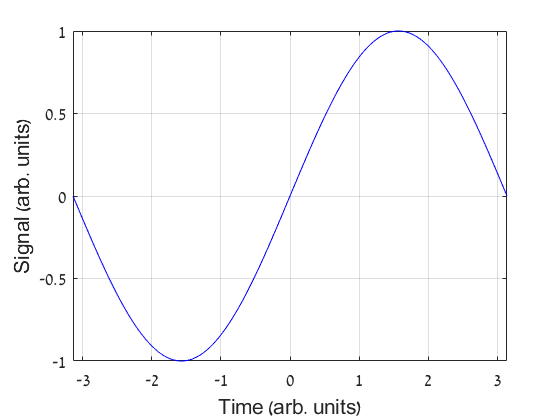
\includegraphics[scale=0.5]{\main/images/chapter_1_example/img_example.png}}
	\caption[Example Image]{Example Image. This image is also labeled internally so we can reference it throughout the text.}
	\label{fig:sine-wave}
\end{figure}
If you want to reference the example figure (Fig.~\ref{fig:sine-wave}), you can. See also Fig.~\ref{fig:cosine-wave}.


\end{document}